\section{Koncept identifikace nejlepší nosnice}\label{sec:koncept-identifikace-nejlepsi-nosnice}
//TODO zkontrolovat pravopis\newline
Při chovu slepic by bylo velmi užitečné vědět, kolik vajec která slepice snáší, protože to umožňuje farmáři sledovat produktivitu jednotlivých slepic.
Díky tomu může:
\begin{itemize}
    \item Optimalizovat chov: Identifikací slepic s vysokou a nízkou snáškou může farmář rozhodnout o selekci nebo o zvláštní péči pro méně produktivní slepice.
    \item Zlepšit zdraví slepic: Nízká snůška může být indikátorem zdravotních problémů.
    Včasná identifikace umožňuje podniknout kroky k léčbě nebo prevenci nemocí.
    \item Efektivněji plánovat krmení a zdroje: Sledování výkonu pomáhá v rozhodování o výživě a péči, aby byla maximalizována produkce vajec při optimálních nákladech.
    \item Zvýšit ziskovost: Monitorováním snůšky lze zlepšit celkovou produktivitu farmy a tím i její ekonomickou efektivitu.
\end{itemize}

Obecně můžeme říci, že znalost počtu snesených vajec od každé slepice pomáhá v efektivním řízení chovu a zajišťuje lepší výsledky, jak po stránce produkční, tak ekonomické.

Abych toho dosáhl, potřebuji být schopen jednotlivé slepice identifikovat a tuto informaci propojit s momentem, kdy slepice snese v hnízdě vejce.
V sekci~\ref{sec:digitalni-vaha-do-hnizda}, je popsán mechanismus, kdy pravidelnou analýzou časové řady, kterou poskytuje váha získáme informaci o časovém údaji, kdy bylo vejce sneseno.
Pak již jen stačí identifikovat, ktera z našich slepic byla v tu dobu v hnízdě.

Existuje několik variant, jak slepice identifikovat, já jsem se rozhodl využít k identifikaci obrazovou analýzu.
Vždycky mě zajímalo na jakém principu funguje rozpoznávání lidí na základě kamerových záznamů, které používá policie případně sledování vozidla, které projíždí nočním městem na červenou skrze několik křižovatek.

Hledání zdrojů na internetu mě přivedlo ke spoustě článků, příspěvků, příkladů i vědeckých prací.

Nakonec jsem nalezl článek~\cite{medium-person-reidentification}, který mě inspiroval. Z článku jsem pochopil základní princip.

Postupuji následujícím způsobem.
Nejprve procházím videozáznam a identifikuji oblasti, kde se slepice nacházejí.
Tyto oblasti následně vystřihnu a uložím do samostatných souborů.
Poté procházím tyto menší obrázky a pomocí segmentace vystřihnu plochu, kde je slepice, zatímco ostatní části zůstanou bílé.
Takto vyříznuté obrázky převádím na tenzory~\cite{Tenzor}.
Převod na tenzor znamená, že dvourozměrný obraz (matice pixelů) převedu do vícerozměrné datové struktury, která dokáže reprezentovat různé vlastnosti obrazu a je vhodná pro strojové učení a další matematické zpracování.
Tímto způsobem získám numerickou reprezentaci obrazu, se kterou mohu efektivně pracovat.
Získané tenzory porovnávám se vzorovými vektory uloženými v databázi.
Pokud je vektor shodný, znamená to, že jsem našel odpovídající slepici, a podařilo se mi ji tak identifikovat.

Algoritmus tedy na počátku vezme jako vstup obrázek z kamery viz obrázek~\ref{fig:source_chick_image}.

\begin{figure}[H]
    \centering
    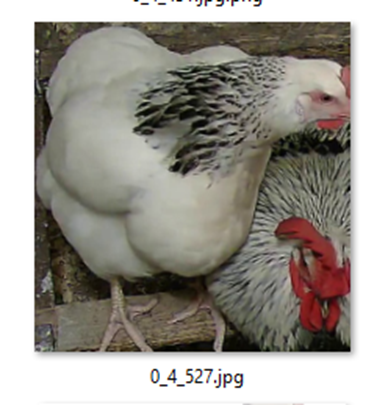
\includegraphics[width=0.8\textwidth]{img/source_chick_image}
    \caption{Jeden ze vstupů do algoritmu pro nosnice}
    \label{fig:source_chick_image}
\end{figure}

Dále je slepice z obrázku vystřižena (segmentována) podle kontury, kterou algoritmus vyhodnotil jako slepice viz obrázek~\ref{fig:segmented_chicks2}.

\begin{figure}[H]
    \centering
    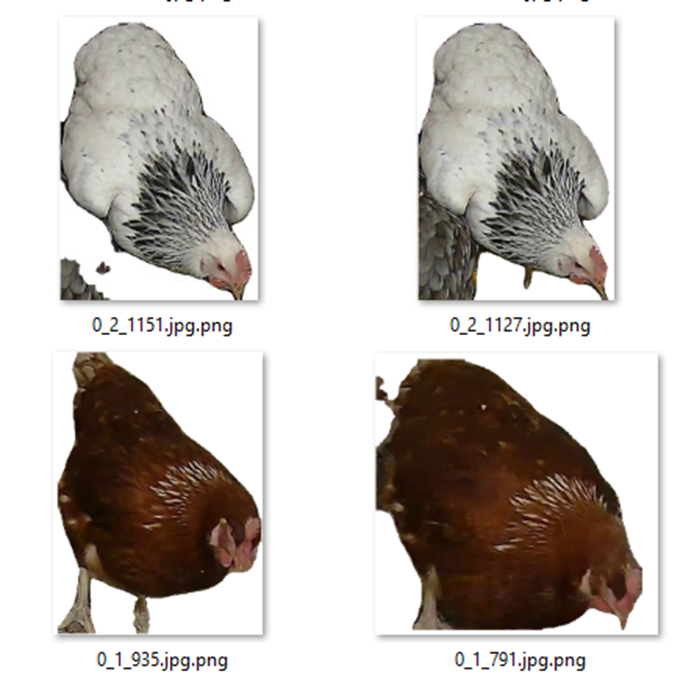
\includegraphics[width=0.8\textwidth]{img/segmented_chicks}
    \caption{Segmentované slepice z fotek}
    \label{fig:segmented_chicks2}
\end{figure}

Na závěr je pro každý výřez vypočítán tenzor (vektor) na jehož základě jsou slepice roztřízeny do jednotlivých skupin viz obrázek~\ref{fig:chicks_in_clusters}.

\begin{figure}[H]
    \centering
    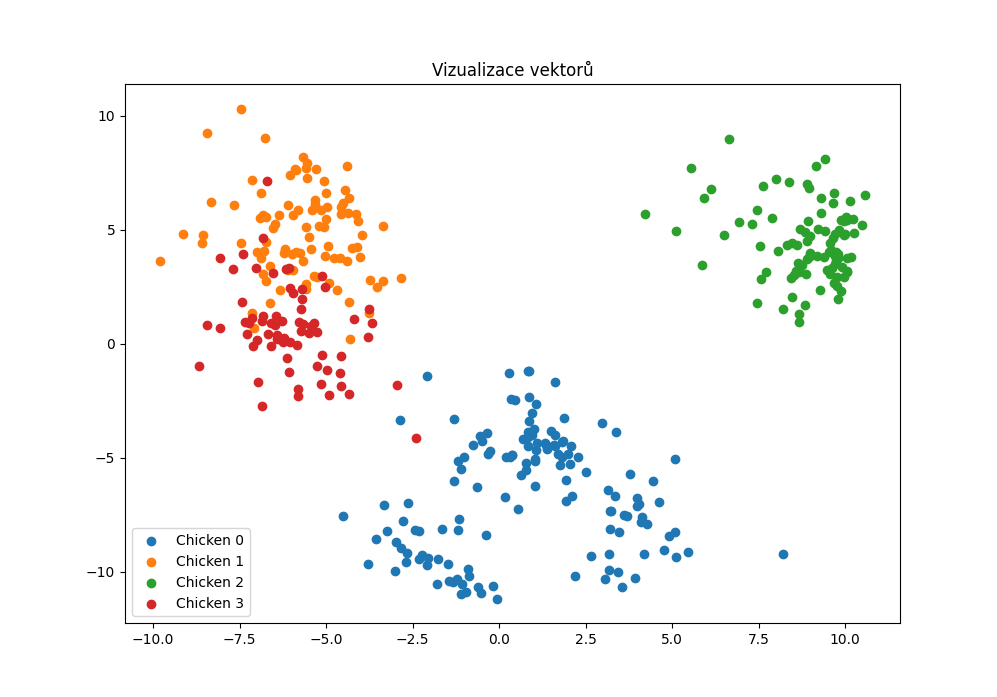
\includegraphics[width=0.8\textwidth]{img/chicks_in_clusters}
    \caption{Algoritmem rozdělené vektory}
    \label{fig:chicks_in_clusters}
\end{figure}

\begin{figure}[H]
    \centering
    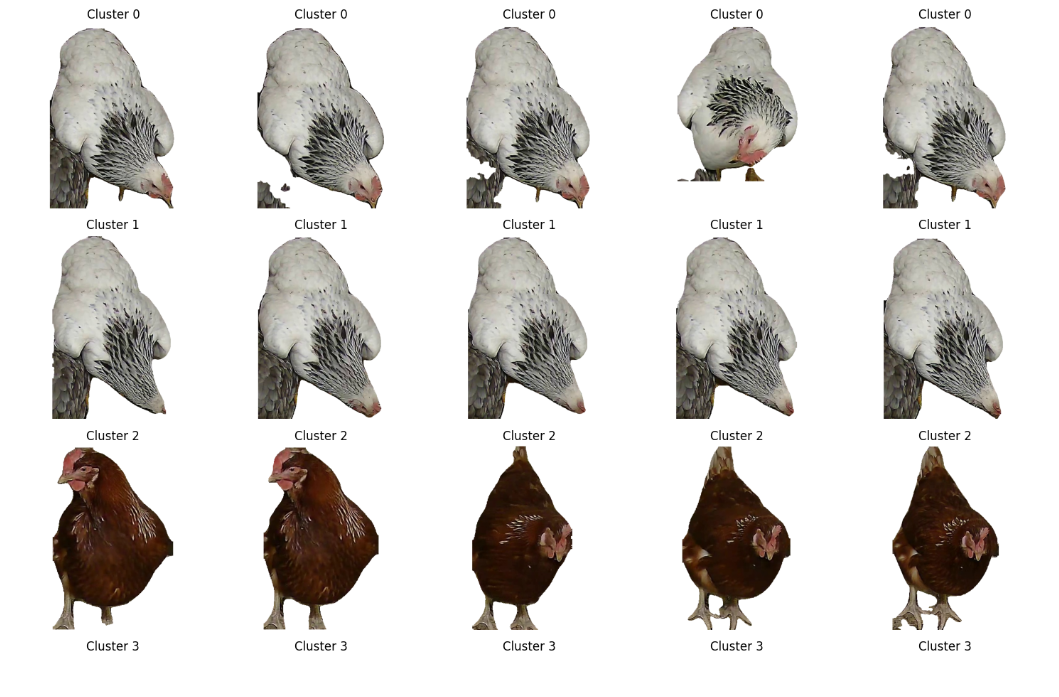
\includegraphics[width=0.8\textwidth]{img/chicks_in_clusters_2}
    \caption{Algoritmem rozdělené slepice}
    \label{fig:chicks_in_clusters_2}
\end{figure}

Během této části projektu, zaměřeného na třídění slepic pomocí umělé inteligence a počítačového vidění, jsem vyvinul základní procesy pro načítání a zpracování obrázků.
Pomocí modelu ResNet50~\cite{ResNet50Documentation} jsem z obrázků extrahoval klíčové vlastnosti a pokusil se slepice zařadit do skupin pomocí metody K-means~\cite{scikit-learnKMeans}.
Bohužel, výsledky zatím nesplnily očekávání.

Hlavním problémem je nedostatečná přesnost klasifikace.
Model má potíže s rozpoznáním rozdílů mezi slepicemi, což vede k logicky nehodnotným skupinám.
Tím ukazuje, že model aktuálně neumí efektivně vyhodnotit důležité charakteristiky pro úspěšné třídění.

Je zřejmé, že projekt vyžaduje další práci.
Potřebuji prozkoumat pokročilejší metody zpracování obrázků a shlukování, případně i techniky hlubokého učení speciálně zaměřené na rozpoznávání zvířat.
Je možné, že bude nutné rozšířit dataset o větší různorodost obrázků a aplikovat techniky, které zlepší schopnost modelu třídit.
Věřím, že s lepšími daty a vylepšeným modelem dosáhnu lepších výsledků.

Při testování na několika obrázcích se zdálo, že by princip mohl fungovat, ale v praxi byl výsledek nepřesný.
Moje babička má dvě červené, dvě bílé a dvě černé slepice, plus jednoho bílého kohouta, což způsobuje, že jsou si slepice často velmi podobné, s nepatrnými rozdíly.

Aktuálně přemýšlím, jak tyto slepice jednoduše odlišit.
Ačkoli pomalování slepic babička pravděpodobně nepovolí, možná by pomohlo zjednodušení úkolu.

Namísto soutěže o nejlepší nosnici bych mohl zaměřit úsilí na sestavení nejefektivnějšího závodního týmu, jako např. týmů bílých, červených nebo černých slepic.





